\subsection{Gameplay Elements}

In this section we will see in more detail all the aspect that make this video games unique in its genre. The game is a 2D single player third person game, the player will play with the character of Minerva, both in her human form and in "cat" form. The combat is turn-based and the formulation of the player's stats are based on the D\&D rules.

%TODO
\paragraph{Exploration Mode}

The player is free to move around  the map in both human form that cat form. If Delphini is also in the player's party, she will follow the player in his every move, but if he is in cat form and enters a place not accessible to humans, Delphini will remain waiting for him When the player is faced with a obstacle, mysterious object or secret passage, he can: 

\begin{itemize}
    \item Use the spells that he has learning to solve the puzzle.
    \item Has the possibility of being able to use the transfiguration to transform small objects into somethings that is needed at the moment.
    \item Transform into cat form and reach places inaccessible to human.
\end{itemize}

The player can interact with NPCs:

\begin{itemize}
    \item In human form he can talk to them, they can make funny story or riddles.
    \item In cat form he can be stroked.
\end{itemize}

\fullwidthgraphicscaption{../Pictures/Gameplay/Dialogue_picture.jpg}{Game: Doom\&Destiny}

\pagebreak 

\paragraph{Combat System}
The combat is turn based. It mostly follows D\&D rules, only exception being that space and movement don't play any role: the combat happens like an old school sideview turn-based rpg. All the D\&D rules that involve moving around don't play any role. Area spells and skills will hit multiple enemies without checking an on-map position. Finally maximum range values for ranged spells and attacks will not play any role.

The main reason is increasing the pace of the fight, since a more complex system which involves movement, getting closer to the turn-based strategy games paradigm, would be too slow paced and complex for the ideal target audience.

\fullwidthgraphicscaption{../Pictures/Gameplay/Combat_picture.png}{Game: Octopath traveler}
\pagebreak

\paragraph{Player rewards}

The player's reward are obtainable in every fight. In the specific combat with Cerberus the player can get: 60 Galleon, 80 Sickle and 100 Knut

\centeredgraphicssize{../Pictures/Gameplay/Rewards_picture.jpg}{5cm}

\paragraph{Experience Points and Friendship Points}

Characters gain Experience Points by completing challenges, missions and minigames (lessons). When Experience Points reach a certain treshold, the Character's level rises. 
Each level grants all the spells of that level which have already been seen during a lesson.

Delphini has an stat in Frienship Points. These increase and decrease depending on the player's choices and successes in missions involving Delphini.

When Delphini is in the party and the friendship level is low, Delphini has access to more aggressive spells, up to Forbidden Curses. 
In contrast, if the friendship level is high, when Minerva attacks Delphini will use a reaction action to perform an attack toghether with Minerva.


\paragraph{Gryffindor Points}

When the player completes a task really well (perfect score in minigames, extremely good timing in timed tasks etcc) or when he fails terribly, some points are added to or removed from the player's House Points. Sometimes player choices can affect the points of other houses as well.
Grants an achievement on the chosen game platform if Gryffindor has the highest points by the end of the game.

\pagebreak 

\paragraph{Checkpoints}

Checkpoints are save points where the player can go back after a defeat. They appear as a Niffler statue which activates when the player makes an offer with a special coine called "Niffler Galleon".
\centeredgraphicssize{../Pictures/Gameplay/Statue_niffler_picture.jpg}{5cm}

\paragraph{Saving}

Checkpoints also save the game. The player can still save at anytime through the main menu. During battles saving is disabled.
\pagebreak

\subsubsection{Items}

\paragraph{Key Items}

\textbf{Key Items}\\

\begin{itemize}
    \item \textbf {Cauldron} 
A tool required in order to prepare potions. A portable version costs 25 galleons, which allows the player to brew potions anywhere. It's magically enchanted to shrink itself so to be easily carried around.
\centeredgraphicssize{../Pictures/Gameplay/Items/Cauldron_picture.png}{5cm}
 
   \item \textbf{Book of Spells }   
A book worth 2 galleons, is used to keep track of the learnt spells.
\centeredgraphicssize{../Pictures/Gameplay/Items/Book_spells_picture.png}{5cm}
   
 \item \textbf{Book of Potions}
 A book worth 2 galleons, is used to keep track of the learnt potion.
\centeredgraphicssize{../Pictures/Gameplay/Items/Book_potions_picture.png}{5cm}
\end{itemize}
\pagebreak



\subparagraph{Currency}

\begin{tabular}{m{3cm}m{3cm}m{6cm} } \hline
	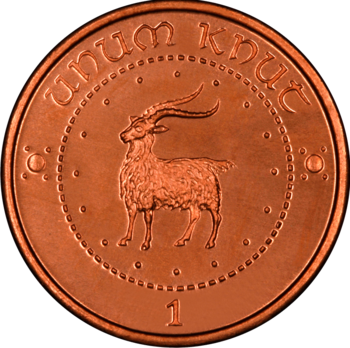
\includegraphics[width=3cm]{../Pictures/Gameplay/Items/Consumables/Currency/Knut_coin_picture.png} & \textbf{Knut} & A Knut, made out of bronze, is the least valued coin in British wizarding currency. There are 29 Knuts in one silver Sickle, and there are 493 Knuts in one golden Galleon. \\ \hline
	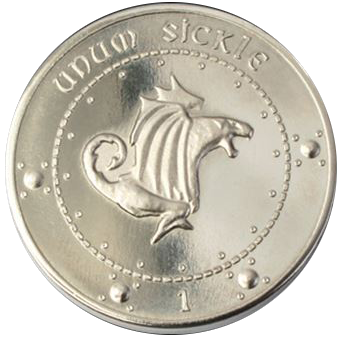
\includegraphics[width=3cm]{../Pictures/Gameplay/Items/Consumables/Currency/Sickle_coin_picture.png} & \textbf{Sickle} & A Sickle, made out of silver, is equal to 29 Knuts, and 17 Sickles make up a Galleon. \\ \hline
	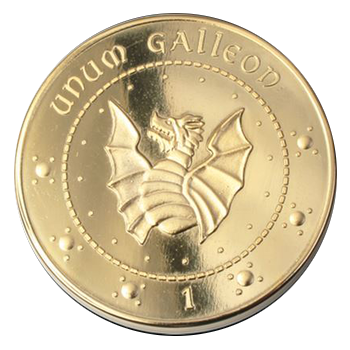
\includegraphics[width=3cm]{../Pictures/Gameplay/Items/Consumables/Currency/Galleon_coin_picture.png} & \textbf{Galleon} & A Galleon, made out of gold, is the most valued coin of the wizarding currency used in Britain. One Galleon is equal to 17 Sickles or 493 Knuts.  \\ \hline
	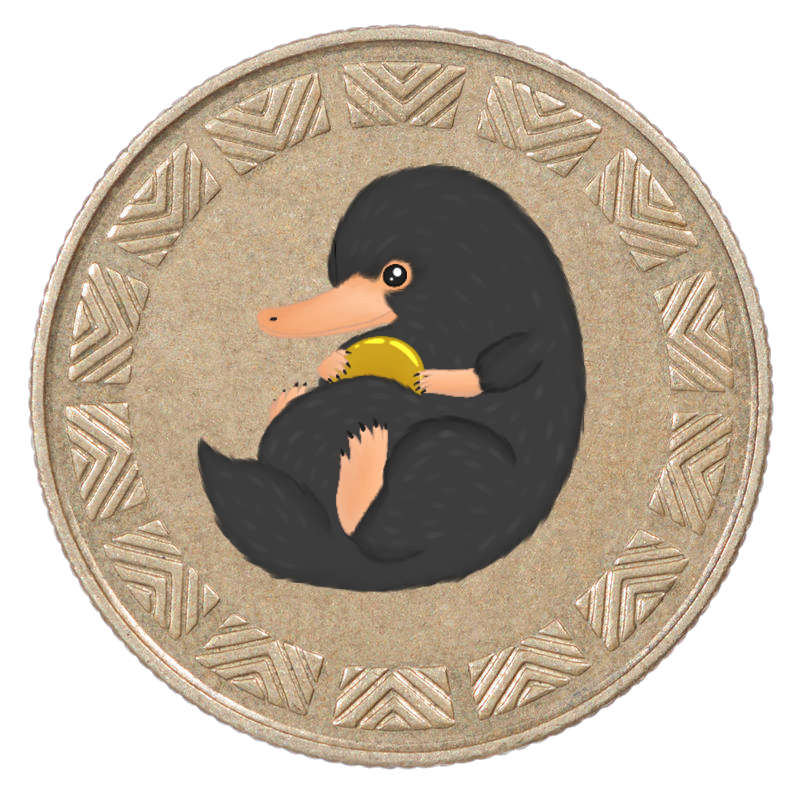
\includegraphics[width=3cm]{../Pictures/Gameplay/Items/Consumables/Currency/Niffler_coin_front_picture.png} & \textbf{Niffler Galleon} & Special currency, grants the blessing of the Niffler when used at their statues, acting as an effective checkpoint for the player. \\ \hline
\end{tabular}

\clearpage


\pagebreak
\paragraph{Consumables}
For consumables we intend all the items that can be used directly or through a crafting process: inside of this category we can find currency, ingredients and craftables. Minerva can carry up to 20 consumable items, but has an unlimited stash in her room, which can be accessed at the beginning of every level, and freely during the Hub Levels. 

\subparagraph{Ingredients}
Ingredients are plants or other elements useful for potion-making.

\begin{tabular}{m{2cm}m{3cm}m{10cm} } 
	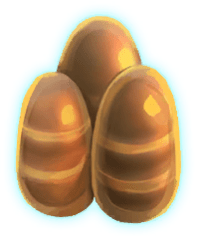
\includegraphics[width=2cm]{../Pictures/Gameplay/Items/Consumables/Ingredients/Ashwinder_eggs_picture.png} & \textbf{Ashwinder Egg} & Ashwinder eggs are the eggs of the Ashwinder , a magical serpent  which is born from the embers of an unattended magical fire. \\ 
	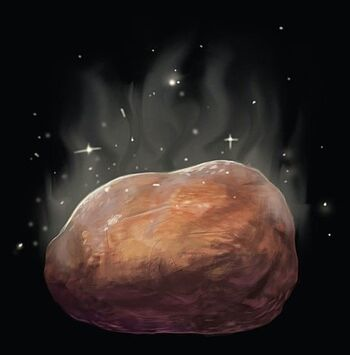
\includegraphics[width=2cm]{../Pictures/Gameplay/Items/Consumables/Ingredients/Bezoar_picture.png} & \textbf{Bezoar} & A bezoar is a stone-like mass taken from the stomach of a goat, that acts as an antitode to most potions \\ 
	
\includegraphics[width=2cm]{../Pictures/Gameplay/Items/Consumables/Ingredients/Bitter_root_picture.png} & \textbf{Bitter Root} & Bitter root (alternatively spelled bitterroot) is a plant that can be used as a potion ingredient. \\ 
	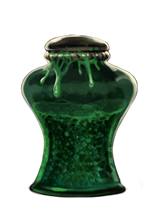
\includegraphics[width=2cm]{../Pictures/Gameplay/Items/Consumables/Ingredients/Flobberworm_mucus_picture.png} & \textbf{Flobberworm Mucus} & Flobberworm mucus, alternatively spelled Flobberworm mucous or Flobber Mucus for short, is the slimy green mucus exuded from the Flobberoworm, often used to thicken potions. \\ 
	
\includegraphics[width=2cm]{../Pictures/Gameplay/Items/Consumables/Ingredients/Granian_hair_picture.png} & \textbf{Granian Hair} & Granian hair is hair taken from a Granian Winged horse, which can be used as a potion ingredient. \\ 
	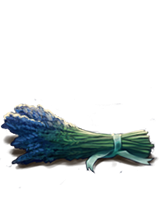
\includegraphics[width=2cm]{../Pictures/Gameplay/Items/Consumables/Ingredients/Lavender_picture.png} & \textbf{Lavender} & Lavender is a flower noted for its "beautiful colour" and "calming fragrance. It can be used as an ingredient in a variety of potions. \\ 
	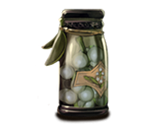
\includegraphics[width=2cm]{../Pictures/Gameplay/Items/Consumables/Ingredients/Mistletoe_berries_picture.png} & \textbf{Mistletoe Berries} & The berry of the mistletoe is small, white, and waxy. It is used as an ingredient in potion. \\ 
	
\includegraphics[width=2cm]{../Pictures/Gameplay/Items/Consumables/Ingredients/Murtlap_tentacle_picture.png} & \textbf{Murtlap Tentacle} & A Murtlap tentacle is a rare potion ingredient that can be obtained from the growth on the back of a Murtlap. \\ 
	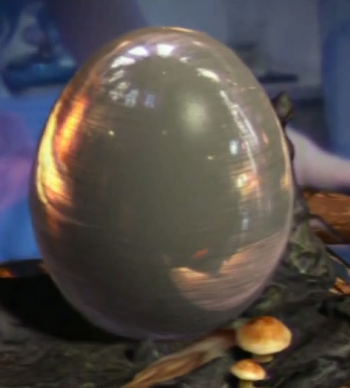
\includegraphics[width=2cm]{../Pictures/Gameplay/Items/Consumables/Ingredients/Occamy_egg_picture.png} & \textbf{Occamy Eggshell} & The egg of the Occamy has a shell made of pure silver, which accounts for why it is so much sought after. \\ 
	
\includegraphics[width=2cm]{../Pictures/Gameplay/Items/Consumables/Ingredients/Reem_blood_picture.png} & \textbf{Re'em Blood} & Re'em blood gives the drinker immense strength for a short time. This in turn makes Re'em blood a highly desired substance, and a useful potion ingredient. \\ 
	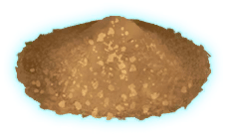
\includegraphics[width=2cm]{../Pictures/Gameplay/Items/Consumables/Ingredients/Rue_picture.png} & \textbf{Rue} & Rue, also known as common rue, is a kind of evergreen shrubs with a distinctive bitter taste. \\ 
	
\includegraphics[width=2cm]{../Pictures/Gameplay/Items/Consumables/Ingredients/Snowdrop_picture.png} & \textbf{Snowdrop} & This plant is very well known for its stimulant properties. \\ 
\end{tabular}

\clearpage

\begin{tabular}{m{2cm}m{3cm}m{10cm} } 
	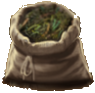
\includegraphics[width=2cm]{../Pictures/Gameplay/Items/Consumables/Ingredients/Standard_ingredient_picture.png} & \textbf{Standard Ingredient} & The Standard Ingredient is a herb, or mixture of dried herbs, with many magical applications and properties that is used as an ingredient in potion-making.  \\ 
	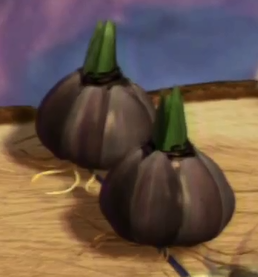
\includegraphics[width=2cm]{../Pictures/Gameplay/Items/Consumables/Ingredients/Squill_bulbs_picture.png} & \textbf{Squill Bulbs} & The bulb of the squill is a structure that functions as an organ for food storage while the plant is dormant. Squill bulbs have potion-making properties and are best harvested just after the plants blossoms. \\ 
	
\includegraphics[width=2cm]{../Pictures/Gameplay/Items/Consumables/Ingredients/Tincture_of_thyme_picture.png} & \textbf{Tincture of Thyme} & Thyme is a common herb with culinary and medicinal uses, making it a good candidate for potion-making. \\ 
	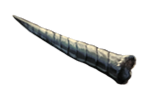
\includegraphics[width=2cm]{../Pictures/Gameplay/Items/Consumables/Ingredients/Unicorn_horn_picture.png} & \textbf{Unicorn Horn} & The horn of a unicorn had magical properties that made it a useful ingredient in potions. \\ 
	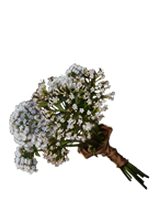
\includegraphics[width=2cm]{../Pictures/Gameplay/Items/Consumables/Ingredients/Valerian_picture.png} & \textbf{Valerian Sprigs} & Valerian is a plant with magical and calming properties. \\ 
\end{tabular}

\clearpage

\subparagraph{Craftables}
Objects made with ingredients\\

\begin{itemize}
    \item \textbf{Antidote common poisons}
 Neutralizes poisonous effects from magical creatures. Can be used both in battle and outside.
 Ingredients: Bezoar, Standard Ingredient, Unicorn Horn, Mistletoe Berries.
\centeredgraphicssize{../Pictures/Gameplay/Items/Consumables/Potions/Antidote_potion_picture.png}{5cm}
    
    \item \textbf{Exstimulo Potion}
Increases the power of spells casted in the next 4 turns.
Ingredients: Re'em blood, Granian hair, Snowdrop and Bitter root
\centeredgraphicssize{../Pictures/Gameplay/Items/Consumables/Potions/Exstimulo_potion_picture.png}{5cm}

    \item \textbf{Felix Felicis}
Makes who drinks it extremely lucky. Combat rewards are increased, healing potions effect is increased, and all rolls are rolled with advantage.
Ingredients: Ashwinder egg, Squill builb, Murtlap tentacle, Tincture of thyme, Occamy eggshell, Powdered common rue.
\centeredgraphicssize{../Pictures/Gameplay/Items/Consumables/Potions/Felix_felicis_potion_picture.png}{5cm}
    
	\item \textbf{Healing Potion}
 Recovers health points. This potion's effect varies based on the amount of ingredients used to prepare it. %TODO: how many ingredients define normal/medium/superior?

\begin{tabular}{ |c|c|c } 
\hline
\textbf{Rarity} & \textbf{HP}  & \textbf{Ingredients Amount} \\
\hline
Normal  & 2d4  & 1  \\
\hline
Medium  & 4d4 & 3 \\
\hline
Superior  & 8d4 & 5 \\
\hline
\end{tabular}

\centeredgraphicssize{../Pictures/Gameplay/Items/Consumables/Potions/Healing_potion_picture.png}{5cm}

	 \item \textbf{Invisibility Potion}
Makes the user invisible. In battle the potion lasts 3 turns, out of battle it lasts one minute. The potion affects the user and everything he's carrying; it terminates when the user attacks, casts a spell, or shifts form.
Ingredients: Flobberworm Mucus, Lavender, Valerian Sprigs, Standard ingredient
\centeredgraphicssize{../Pictures/Gameplay/Items/Consumables/Potions/Invisibility_potion_picture.png}{5cm}
\end{itemize}
\pagebreak

\paragraph{Wands}
\textbf{Wands} In Hogwarts, everything is based on wizardry and spells: for this reason the wand, together with protective jewelry, will play an important role in combat, enhancing the magical capabilities of our characters in different ways.

The wand is the most important tool in a wizard's life: inner magical power is channeled through it and it can cast any kind of spell. Each wand is made of wood and contains an enchanted core, a special material usually coming from magical creatures.
\centeredgraphicssize{../Pictures/Gameplay/Items/Wand_picture.jpg}{5cm}
There are several types of wand wood and cores, which will alter and enhance the capabilities of the wielder.

\paragraph{Wood} The wood will grant a bonus to its particular category of spells: \\

\begin{tabular}{ m{4cm}m{3cm}m{6cm} } \hline
	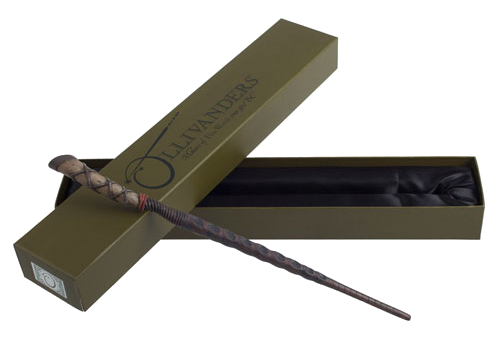
\includegraphics[width=4cm]{../Pictures/Gameplay/Items/Wearables/Wand/Wood/Holly_wood_picture.png} & \textbf{Holly} & Holly will boost defensive spells, naturally meant for casters who think that a good defense is the best offense. \\ \hline
	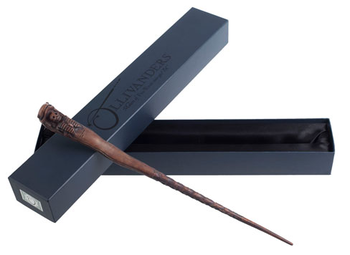
\includegraphics[width=4cm]{../Pictures/Gameplay/Items/Wearables/Wand/Wood/Alder_wood_picture.png} & \textbf{Alder} & Alder will boost buff spells, aiding mages who seek to help and empower others. \\ \hline
	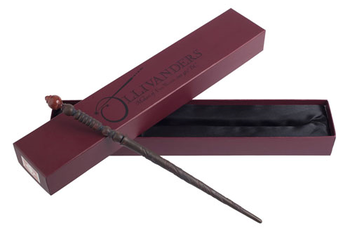
\includegraphics[width=4cm]{../Pictures/Gameplay/Items/Wearables/Wand/Wood/Cedar_wood_picture.png} & \textbf{Cedar} & Cedar will boost debuff spells, perfect for wizards who prefer to weaken their enemies before striking.  \\ \hline
	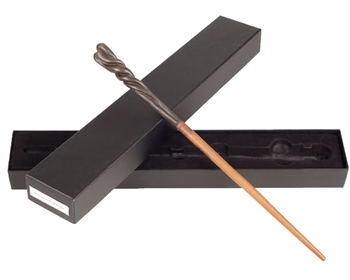
\includegraphics[width=4cm]{../Pictures/Gameplay/Items/Wearables/Wand/Wood/Cherry_wood_picture.png} & \textbf{Cherry} & Cherry will boost attack spells, favored by sorcerers who follow the rule "strike first, strike hard". \\ \hline
	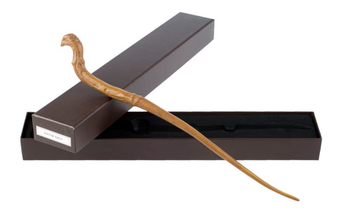
\includegraphics[width=4cm]{../Pictures/Gameplay/Items/Wearables/Wand/Wood/Pine_wood_picture.png} & \textbf{Pine} & Pine will boost utility spells, preferred by creative enchanters and out-of-the-box thinkers. \\ \hline
\end{tabular}
\pagebreak 
\begin{itemize}
    \item The bonus for non-Utility category will make spells of that category cast as 1 level higher (if applicable).
    \item The bonus for Utility category will grant an extra spell slot reserved to Utility spells for each spell level the character has access to.
\end{itemize}

\clearpage


\paragraph{Cores}
Cores will grant an unique bonus feat \\

\begin{tabular}{ m{4cm}m{3cm}m{6cm} } \hline
	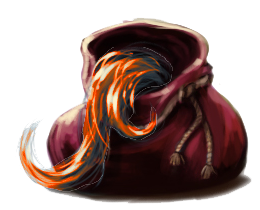
\includegraphics[width=4cm]{../Pictures/Gameplay/Items/Wearables/Wand/Cores/Dragon_heartstring_icon.png} & \textbf{Dragon Heartstring (Dual wielder)} & You can equip a second wand. You get the bonus from the wood of that wand, but not from its core. \\ \hline
	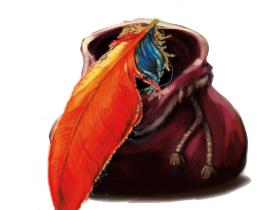
\includegraphics[width=4cm]{../Pictures/Gameplay/Items/Wearables/Wand/Cores/Phoenix_feather_icon.png} & \textbf{Phoenix Feather (Alert)} & Adds +5 to Initiative. \\ \hline
	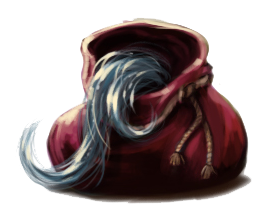
\includegraphics[width=4cm]{../Pictures/Gameplay/Items/Wearables/Wand/Cores/Unicorn_hair_icon.png} & \textbf{Unicorn Hair (Resilient)} & Adds +1 in one ability score and you gain proficiency in saving throws using that ability.  \\ \hline
	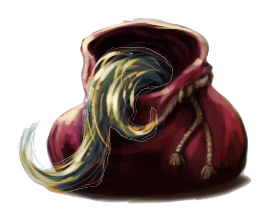
\includegraphics[width=4cm]{../Pictures/Gameplay/Items/Wearables/Wand/Cores/Veela_hair_icon.png} & \textbf{Veela Hair (Healer)} & You can stabilize a creature and restore it to 1 hp, or restore [1d6+4+its number of Hit Dice] hp to it; can't be used more than once per day on the same creature. \\ \hline
	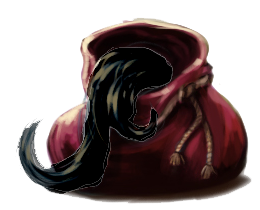
\includegraphics[width=4cm]{../Pictures/Gameplay/Items/Wearables/Wand/Cores/Thestral_tail_hair_icon.png} & \textbf{Thestral Tail Hair (Lucky)} & You can reroll a d20 or force to reroll an attack roll against you. Can be used up to 3 times per day. \\ \hline
\end{tabular}

\clearpage

\paragraph{Amulets}
Amulets will enhance ability scores \\

\begin{tabular}{m{2cm}m{3cm}m{4cm} } 
	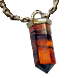
\includegraphics[width=2cm]{../Pictures/Gameplay/Items/Wearables/Amulets/Amber_amulet_icon.png} & \textbf{Amber} & adds +1 STR \\ 
	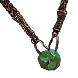
\includegraphics[width=2cm]{../Pictures/Gameplay/Items/Wearables/Amulets/Jade_amulet_icon.png} & \textbf{Jade} & adds +1 DEX \\ 
	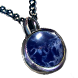
\includegraphics[width=2cm]{../Pictures/Gameplay/Items/Wearables/Amulets/Lapis_amulet_icon.png} & \textbf{Lapis} & adds +1 INT \\ 
	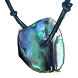
\includegraphics[width=2cm]{../Pictures/Gameplay/Items/Wearables/Amulets/Paua_amulet_icon.png} & \textbf{Paua} & adds +1 WIS \\ 
	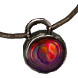
\includegraphics[width=2cm]{../Pictures/Gameplay/Items/Wearables/Amulets/Coral_amulet_icon.png} & \textbf{Coral} & adds +1 CON \\ 
	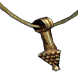
\includegraphics[width=2cm]{../Pictures/Gameplay/Items/Wearables/Amulets/Gold_amulet_icon.png} & \textbf{Gold} & adds +1 CHA \\ 
	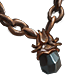
\includegraphics[width=2cm]{../Pictures/Gameplay/Items/Wearables/Amulets/Onyx_amulet_icon.png} & \textbf{Onyx} & (Rare), adds +1 to all ability scores 
\end{tabular}

\clearpage

\paragraph{Rings}

Rings will grant an unique bonus to the wearer. One can wear maximum two rings at once.
\begin{itemize}

    \item \textbf{Paua},  gives 1 additional spell slot, usable by any spell of any level
\centeredgraphicssize{../Pictures/Gameplay/Items/Wearables/Rings/Paua_ring_icon.png}{5cm}

  \item \textbf{Coral}, adds +8 HP
\centeredgraphicssize{../Pictures/Gameplay/Items/Wearables/Rings/Coral_ring_icon.png}{5cm}

  \item \textbf{Moonstone}, adds +2 on CA and +2 on Saving Throws when defending against spell attacks.
\centeredgraphicssize{../Pictures/Gameplay/Items/Wearables/Rings/Moonstone_ring_icon.png}{5cm}

  \item \textbf{Diamond} , adds +2 CA when defending against physical attacks.
\centeredgraphicssize{../Pictures/Gameplay/Items/Wearables/Rings/Diamond_ring_icon.png}{5cm}

\end{itemize}
\pagebreak

\pagebreak
\subsection{Spells}
A spell is a controlled manifestation of magic expressed through wand movement, incantation words, concentration and intention. For this reason, all spells only require for Vocal and Somatic elements to be casted. \\


\paragraph{Attack} 
Spells specialized for offensive purposes. \\

\subparagraph{Level 0} 
Common spells \\
\begin{tabular}{ m{2cm}m{3cm}m{4cm}m{6cm} } 
	
\includegraphics[width=2cm]{../Pictures/Gameplay/Spells/Icon/Stupeficium_spell_icon.png} & \textbf{Stupeficium} & Hits the target with a swift bolt of stunning energy. & Make a ranged spell attack against the target. On a hit, the target takes 1d10 force damage. This spell's damage increases by 1d10 when you reach 5th level (2d10), 11th level (3d10), and 17th level (4d10). \\ 
\end{tabular}

\subparagraph{Level 1} 
Low level spells \\
\begin{tabular}{ m{2cm}m{3cm}m{4cm}m{6cm} } 
	
\includegraphics[width=2cm]{../Pictures/Gameplay/Spells/Icon/Incendio_spell_icon.png} & \textbf{Incendio} & Produces a cone of fire from the tip of the wand. & A creature and its neighbours make a DEX saving throw: each takes 3d6 fire damage on a failed save, or half as much damage on a successful one.  \\ 
	
\includegraphics[width=2cm]{../Pictures/Gameplay/Spells/Icon/Baubillious_spell_icon.png} & \textbf{Baubillious} & Produces a bolt of white light as a wave of thunderous force sweeps out from you. & A creature and its neighbours make a CON saving throw: each takes 2d8 thunder damage and is knocked prone on a failed save, or only half as much damage on a successful one.\\
	\includegraphics*[width=2cm]{../Pictures/Gameplay/Spells/Icon/Sectumsempra_spell_icon.png} & \textbf{Sectumsempra} & Lacerates the target, as if they have been slashed by a sword. & Make a melee spell attack against a creature you choose. On a hit, the target takes 3d10 damage. \\
\end{tabular}

\subparagraph{Level 3} 
Medium spells \\
\begin{tabular}{ m{2cm}m{3cm}m{4cm}m{6cm} } 
	
\includegraphics[width=2cm]{../Pictures/Gameplay/Spells/Icon/Glacius_spell_icon.png} & \textbf{Glacius} & Freezes the target with icy-cold air. & Each enemy creature must make a CON saving throw: each takes 4d8 cold damage on a failed save, or half as much damage on a successful one. \\ 
	
\includegraphics[width=2cm]{../Pictures/Gameplay/Spells/Icon/Aqua_Eructo_spell_icon.png} & \textbf{Aqua eructo} & Create, and control, a wave of water from the tip of the wand. & Each enemy creature must make a DEX saving throw: each takes 4d8 bludgeoning damage and is knocked prone on a failed save, or only half as much damage on a successful one.  \\ 
	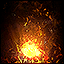
\includegraphics[width=2cm]{../Pictures/Gameplay/Spells/Icon/Bombarda_spell_icon.png} & \textbf{Bombarda} & Provokes a small but fiery heat explosion. & A creature and its neighbours make a DEX saving throw: each takes 8d6 fire damage on a failed save, or half as much damage on a successful one.\\ 
\end{tabular}

\subparagraph{Level 5} 
Greater spells \\
\begin{tabular}{ m{2cm}m{3cm}m{4cm}m{6cm} } 
	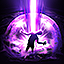
\includegraphics[width=2cm]{../Pictures/Gameplay/Spells/Icon/Expulso_spell_icon.png} & \textbf{Expulso} &  Provokes a pressure explosion, instead of a heat one. & Each enemy creature must make a CON saving throw: each takes 5d6 thunder damage + 5d6 radiant(or necrotic) damage and is knocked on a failed save, only half as much damage on a successful save. \\ 
	
\includegraphics[width=2cm]{../Pictures/Gameplay/Spells/Icon/Immobilus_spell_icon.png} & \textbf{Immobilus} & Immobilises and stops the actions of the targets with extreme cold. & A creature and its neighbours make a CON saving throw: each takes 8d8 cold damage on a failed save, or half as much damage on a successful one.\\
	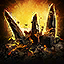
\includegraphics[width=2cm]{../Pictures/Gameplay/Spells/Icon/Dominusterrae_spell_icon.png} & \textbf{Dominusterrae} & A fountain of churned earth and stone erupts from where your wand is pointing at. & Each enemy creature must make a DEX saving throw. A creature takes 5d12 bludgeoning damage and is knocked on a failed save, or take only half as much damage on a successful one.\\ 
\end{tabular}

\subparagraph{Level 7} 
Superior spells \\
\begin{tabular}{ m{2cm}m{3cm}m{4cm}m{6cm} } 
	
\includegraphics[width=2cm]{../Pictures/Gameplay/Spells/Icon/Crucio_spell_icon.png} & \textbf{Crucio} & Inflicts intense pain on the recipient of the curse. & The target must make a CON saving throw: it takes 7d8 + 30 necrotic damage on a failed save, or half as much damage on a successful one.\\ 
	
\includegraphics[width=2cm]{../Pictures/Gameplay/Spells/Icon/Fiendfyre_spell_icon.png} & \textbf{Fiendfyre} & Unleashes cursed fire that takes the shape of animals that actively seek out living targets and burn anything in its path. & Each targeted enemy must make a DEX saving throw: each takes 7d10 fire damage on a failed save, or half as much damage on a successful one.  \\ 
\end{tabular}

\subparagraph{Level 8} 
Supreme spells \\
\begin{tabular}{ m{2cm}m{3cm}m{4cm}m{6cm} } 
	\includegraphics[width=2cm]{../Pictures/Gameplay/Spells/Icon/Lumos_Solem_spell_icon.png} & \textbf{Lumos Solem} & Produce a blinding flash of sunlight. & Each enemy creature makes a CON saving throw: on a failed save, a creature takes 12d6 radiant damage and is blinded for 2 turns, only half as much damage on a successful one \\ 
	\includegraphics[width=2cm]{../Pictures/Gameplay/Spells/Icon/Avada_Kedavra_spell_icon.png} & \textbf{Avada Kedavra} & Causes instantaneous death. It is accompanied by a flash of green light and a rushing noise. & If the creature you choose has 100 hit points or fewer, it dies. Otherwise, the spell has no effect. \\ 
	\includegraphics[width=2cm]{../Pictures/Gameplay/Spells/Icon/Jelly_Brain_spell_icon.png} & \textbf{Jelly-Brain Jinx} & Reduces the target's mental processes. & The target takes 4d6 psychic damage and must make an INT saving throw: on a failed save, the targed is stunned for 3 turns.\\ 
\end{tabular}
\pagebreak








\paragraph{Def} 

\textbf{Level 0} 
\begin{tabular}{ m{4cm}m{3cm}m{6cm} } 
	\includegraphics[width=4cm]{../Pictures/Gameplay/Spells/Icon/spell_icon.png} & \textbf{Protego minima} & A powerful shield charm against dark magic. Once before the spell ends, the target can roll a d4 and add the number rolled to one saving throw of its choice. It can roll the die before or after making the saving throw. The spell then ends \\ 
\end{tabular}
\textbf{Level 1} 
\begin{tabular}{ m{4cm}m{3cm}m{6cm} } 
	\includegraphics[width=4cm]{../Pictures/Gameplay/Spells/Icon/spell_icon.png} & \textbf{Ferula} & Conjures up bandages and wraps them around a wound, splinting any broken bones. Of hit points equal to 1d8 + your spellcasting ability modifier\\ 
   \includegraphics[width=4cm]{../Pictures/Gameplay/Spells/Icon/spell_icon.png} & \textbf{Protego} &  The target's base AC becomes 13 + its Dexterity modifier. The spell ends if the target dons armor or if you dismiss the spell as an action. \\ 
\end{tabular}
\textbf{Level 3} 
\begin{tabular}{ m{4cm}m{3cm}m{6cm} } 
%todo
	\includegraphics[width=4cm]{../Pictures/Gameplay/Spells/Icon/spell_icon.png} & \textbf{Finite Incantatum} & Terminates all spell effects in the vicinity of the caster. \\ 
   \includegraphics[width=4cm]{../Pictures/Gameplay/Spells/Icon/spell_icon.png} & \textbf{Episkey} & Used to heal relatively minor injuries, such as broken bones and cartilage. As you call out words of restoration, up to six creatures of your choice that you can see within range regain hit points equal to 1d4 + your spellcasting ability modifier.\\ 
\end{tabular}
\textbf{Level 5 } 
\begin{tabular}{ m{4cm}m{3cm}m{6cm} } 
	\includegraphics[width=4cm]{../Pictures/Gameplay/Spells/Icon/spell_icon.png} & \textbf{Expecto Patronum} & This charm is a highly powerful and advanced protective spell which will conjure a spirit guardian of their positive emotions to defend against dark creatures.  \\  % todo 
	\includegraphics[width=4cm]{../Pictures/Gameplay/Spells/Icon/spell_icon.png} & \textbf{Re-enervate} & Awakens an unconscious victim. It is consequently the counter-charm to the Stunning Spell. That creature returns to life with 1 hit point. This spell can't return to life a creature that has died of old age, nor can it restore any missing body parts. \\ 
\end{tabular}
\textbf{Level 7} 
\begin{tabular}{ m{4cm}m{3cm}m{6cm} } 
	\includegraphics[width=4cm]{../Pictures/Gameplay/Spells/Icon/spell_icon.png} & \textbf{Vulnera Sanentur} & Healing spell that slows blood flow, clears residue, and knits wounds. The target regains 4d8 + 15 hit points. For the duration of the spell, the target regains 1 hit point at the start of each of its turns  \\ 
\end{tabular}
\textbf{Level 8} 
\begin{tabular}{ m{4cm}m{3cm}m{6cm} } 
	\includegraphics[width=4cm]{../Pictures/Gameplay/Spells/Icon/spell_icon.png} & \textbf{Protego Maxima} & Any spell of 5th level or lower cast from outside the barrier can't affect creatures or objects within it, even if the spell is cast using a higher level spell slot. Such a spell can target creatures and objects within the barrier, but the spell has no effect on them. Similarly, the area within the barrier is excluded from the areas affected by such spells. \\ 
\end{tabular}

\pagebreak













\paragraph{Buff} 
Spells specialized for aiding and empowering others. \\


\subparagraph{Level 0} 
Common spells \\
\begin{tabular}{ m{2cm}m{3cm}m{4cm}m{6cm} } 
	\includegraphics[width=2cm]{../Pictures/Gameplay/Spells/Icon/Revelio_minima_spell_icon.jpg} & \textbf{Revelio minima} & Reveals secrets about a person or object. Your magic grants you a brief insight into the target's defenses. & On your next turn, you gain advantage on your first attack roll against the target, provided that this spell hasn't ended. \\ 
   \includegraphics[width=2cm]{../Pictures/Gameplay/Spells/Icon/Inveterasco_spell_icon.png} & \textbf{Inveterasco} & Helps the caster focus better on his current task & Once before the spell ends, the target of the spell can roll a d4 and add the number rolled to one ability check of its choice. The spell then ends. \\ 
\end{tabular}

\subparagraph{Level 1} 
Low level spells \\
\begin{tabular}{ m{2cm}m{3cm}m{4cm}m{6cm} } 
	\includegraphics[width=2cm]{../Pictures/Gameplay/Spells/Icon/Empowering_spell_icon.png} & \textbf{Empowering Charm} & Invigorates the spirits of the targets of this spell. & Whenever a target makes an attack roll or a saving throw before the spell ends, the target can roll a d4 and add the result to his attack roll or saving throw. \\ %todo %todo ask why this todo is here 
\includegraphics[width=2cm]{../Pictures/Gameplay/Spells/Icon/Engorgio_spell_icon.png} & \textbf{Engorgio / Reducio} & Causes the target to swell or dwindle in physical size. & \textbf{Enlarged}: dimensions doubled, adv. in STR checks and saving throws, +1d4 to target weapons. \textbf{Reduced}: dimensions halved, disadv. in STR checks and saving throws, -1d4 to target weapons (can't be less than 1).  \\ 
\end{tabular}

\subparagraph{Level 3} 
Medium spells \\
\begin{tabular}{ m{2cm}m{3cm}m{4cm}m{6cm} } 
	\includegraphics[width=2cm]{../Pictures/Gameplay/Spells/Icon/Haste_spell_icon.png} & \textbf{Quickening Charm} & Makes a target hasten its movements and thoughts. & Choose a willing creature that you can see within range. Until the spell ends, the target's speed is doubled, it gains a +2 bonus to AC, it has advantage on Dexterity saving throws, and it gains an additional action on each of its turns. \\ 
   \includegraphics[width=2cm]{../Pictures/Gameplay/Spells/Icon/Heroism_spell_icon.png} & \textbf{Power of Belief } & Imbues the target of the spell with unprecedented bravery & Until the spell ends, up to three creatures are immune to being frightened and gain temporary hit points equal to your spellcasting ability modifier at the start of each of its turns. When the spell ends, the targets lose any remaining temporary hit points from this spell. \\  
\end{tabular}

\subparagraph{Level 5} 
Greater spells \\
\begin{tabular}{ m{2cm}m{3cm}m{4cm}m{6cm} } 
	\includegraphics[width=2cm]{../Pictures/Gameplay/Spells/Icon/Salvio_Hexia_spell_icon.png} & \textbf{Salvio Hexia} & Makes an area magically secure, protecting against hexes and spells. &  The spell prevents any physical or magical method from seeing what's inside of the secured area from the outside. \\ 
\end{tabular}

\subparagraph{Level 7} 
Superior spells \\
\begin{tabular}{ m{2cm}m{3cm}m{4cm}m{6cm} } 
	\includegraphics[width=2cm]{../Pictures/Gameplay/Spells/Icon/Occlumency_spell_icon.png} & \textbf{Occlumency} & Prevents legilimency and other harming effects on the mind. & Until the spell ends, one willing creature you touch is immune to psychic damage, any effect that would sense its emotions or read its thoughts, divination spells, and the charmed condition. \\ 
\end{tabular}

\subparagraph{Level 8} 
Supreme spells \\
\begin{tabular}{ m{2cm}m{3cm}m{4cm}m{6cm} } 
	\includegraphics[width=2cm]{../Pictures/Gameplay/Spells/Icon/Righteous_aura_spell_icon.png} & \textbf{Righteous aura} & Invigorating light washes out around the caster. & Each creature chosen by the caster around him has advantage on all saving throws and other creatures has disavantage on attack rolls on them. The attacker must succeed on a CON saving throw or be blinded for 1 turn. \\ 
\end{tabular}

\pagebreak
















\paragraph{Debuff} 


\subparagraph{Level 0} 
Common spells \\
\begin{tabular}{ m{2cm}m{3cm}m{4cm}m{6cm} } 
	\includegraphics[width=2cm]{../Pictures/Gameplay/Spells/Icon/Expelliarmus_spell_icon.png} & \textbf{Expelliarmus} &  Forces whatever an opponent is holding to fly out of their hand. & Until the end of your next turn, you have resistance against bludgeoning, piercing, and slashing damage dealt by weapon attacks.  \\ 
\end{tabular}


\subparagraph{Level 1} 
 Low  spells\\
\begin{tabular}{ m{2cm}m{3cm}m{4cm}m{6cm} } 
	\includegraphics[width=2cm]{../Pictures/Gameplay/Spells/Icon/Somnus_spell_icon.png} & \textbf{Somnus} & Produce a sweet sound that puts your opponent to sleep & Roll 5d8; the total is how many hit points of creatures this spell can affect. \\

	\includegraphics[width=2cm]{../Pictures/Gameplay/Spells/Icon/Petrificus_spell_icon.png} & \textbf{Petrificus} &It is a curse that has temporarily paralyzed the opponent. & The target must succeed on a Wisdom saving throw or be paralyzed for the duration. At the end of each of its turns, the target can make another Wisdom saving throw. If successful, the spell ends on the target.\\ 
	
\includegraphics[width=2cm]{../Pictures/Gameplay/Spells/Icon/spell_icon.png} & \textbf{Rictumsempra} & Tickles the target until they become weak with laughter. & The target must succeed on a Wisdom saving throw or fall prone, becoming incapacitated and unable to stand up for the duration. A creature with an Intelligence score of 4 or less isn't affected.\\ 
\end{tabular}

\subparagraph{Level 3} 
Medium  spells\\
\begin{tabular}{ m{2cm}m{3cm}m{4cm}m{6cm} } 
	\includegraphics[width=2cm]{../Pictures/Gameplay/Spells/Icon/Impendimenta_spell_icon.png} & \textbf{Impendimenta} & Slows down or stops the target. & Change the time of up to 6 creatures on the field. Each target must succeed on a Wisdom saving throw or be affected by this spell for the duration. \\ 

\includegraphics[width=2cm]{../Pictures/Gameplay/Spells/Icon/Obscuro_spell_icon.png} & \textbf{Obscuro} & You can blind or deafen a foe. & Choose one creatur to make a Constitution saving throw. If it fails, the target is either blinded or deafened  for the duration. At the end of each of its turns, the target can make a Constitution saving throw. On a success, the spell ends. \\ 

\includegraphics[width=2cm]{../Pictures/Gameplay/Spells/Icon/Weakening_spell_icon.png} & \textbf{Weakening Hex} & Causes brooms to vibrate violently in the air and try to buck their rider off. &  Up to three creatures must make Charisma saving throws. Whenever a target that fails this saving throw makes an attack roll or a saving throw before the spell ends, the target must roll a d4 and subtract the number rolled from the attack roll or saving throw.\\ 
\end{tabular}


\subparagraph{Level 5} 
Greater spells\\
\begin{tabular}{ m{2cm}m{3cm}m{4cm}m{6cm} } 

	\includegraphics[width=2cm]{../Pictures/Gameplay/Spells/Icon/Confundo_spell_icon.png} & \textbf{Confundo} & Causes the victim to become confused and befuddled. &  roll d10
1-6 The creature takes no action this turn.
7-10 The creature can move normally. 
\\ 
	\includegraphics[width=2cm]{../Pictures/Gameplay/Spells/Icon/Petrificus_Totalus_spell_icon.png} & \textbf{Petrificus Totalus} & . The target must succeed on a Wisdom saving throw or be paralyzed for the duration \\ 
\end{tabular}


\subparagraph{Level 7} 
Superior  spells\\
\begin{tabular}{ m{2cm}m{3cm}m{4cm}m{6cm} } 
	\includegraphics[width=2cm]{../Pictures/Gameplay/Spells/Icon/Mantra_spell_icon.png} & \textbf{Mantra} & You utter a divine word, imbued with the power that shaped the world at the dawn of creation & Each creature that can hear you must make a Charisma saving throw. On a failed save, a creature suffers an effect based on its current hit points \\
\end{tabular}

\subparagraph{Level 8} 
Low level spells \\
\begin{tabular}{ m{2cm}m{3cm}m{4cm}m{6cm} } 
	\includegraphics[width=4cm]{../Pictures/Gameplay/Spells/Icon/Imperio_spell_icon.png} & \textbf{Imperio} & Places the victim completely under the caster's control.  & You try to deceive a creature. He must succeed on a Wisdom saving throw or be fascinated by you for the duration. If you or your partner are fighting him, he has the advantage on the saving throw. \\ 
\end{tabular}
\pagebreak















\paragraph{Utility} 
Multi-purpose spells that can be used in very creative ways. 

\subparagraph{Level 0} 
Common spells \\
\begin{tabular}{ m{2cm}m{3cm}m{8cm}} 
  \includegraphics[width=2cm]{../Pictures/Gameplay/Spells/Icon/Lumos_spell_icon.png} & \textbf{Lumos} & Illuminates the tip of the caster's wand, allowing the caster to see in the dark. The spell ends if you cast it again or dismiss it as an action.\\ 
	\includegraphics[width=2cm]{../Pictures/Gameplay/Spells/Icon/Reparo_spell_icon.png} & \textbf{Reparo} & Seamlessly repairs broken objects. This spell repairs a single break or tear in an object you touch, such as a broken chain link, two halves of a broken key, a torn cloak, or a leaking wineskin \\ 
	\includegraphics[width=2cm]{../Pictures/Gameplay/Spells/Icon/Accio_spell_icon.png} & \textbf{Accio} &  Summons a familiar object towards the caster by describing it or naming it. \\ 
\end{tabular}

\subparagraph{Level 1} 
 Low level spells\\
\begin{tabular}{ m{2cm}m{3cm}m{8cm} } 
 \includegraphics[width=2cm]{../Pictures/Gameplay/Spells/Icon/Wingardium_spell_icon.png} & \textbf{Wingardium Leviosa} & Makes objects fly, or levitate.   \\ 
	\includegraphics[width=2cm]{../Pictures/Gameplay/Spells/Icon/Fumos_spell_icon.png} & \textbf{Fumos} & It's a charm used to create a defensive cloud of smoke from the wand that hinders visibility. \\  
\end{tabular}

\subparagraph{Level 3} 
Medium spells\\
\begin{tabular}{ m{2cm}m{3cm}m{8cm} } 
	\includegraphics[width=2cm]{../Pictures/Gameplay/Spells/Icon/Alomohora_spell_icon.png} & \textbf{Alomohora} & Unlocks doors and other locked objects. \\ 
   \includegraphics[width=2cm]{../Pictures/Gameplay/Spells/Icon/Colloportus_spell_icon.png} & \textbf{Colloportus} & Locks doors and all things that can be locked. \\ 
\end{tabular}
	

\subparagraph{Level 5} 
Greater spells\\
\begin{tabular}{ m{2cm}m{3cm}m{8cm} } 
	\includegraphics[width=2cm]{../Pictures/Gameplay/Spells/Icon/Revelio_spell_icon.jpg} & \textbf{Revelio} & Reveals secrets and occulted information about a person or object.  \\ 
	\includegraphics[width=2cm]{../Pictures/Gameplay/Spells/Icon/Transfiguration_spell_icon.png} & \textbf{Transfiguration} & This spell transforms a creature or an object that you can see within range into a new form. An unwilling creature must make a Wisdom saving throw to avoid the effect. \\ 
\end{tabular}


\subparagraph{Level 7} 
Superior spells\\
\begin{tabular}{ m{2cm}m{3cm}m{8cm} } 
	\includegraphics[width=2cm]{../Pictures/Gameplay/Spells/Icon/Apparate_spell_icon.png} & \textbf{Apparate} & Magically transports the caster to another location instantaneously.  \\ 
\end{tabular}

\subparagraph{Level 8} 
Supreme spells \\
\begin{tabular}{ m{2cm}m{3cm}m{8cm} } 
  	\includegraphics[width=2cm]{../Pictures/Gameplay/Spells/Icon/Portkey_spell_icon.png} & \textbf{Portkey} & Turns an object into a portkey.\\ 
\end{tabular}


\pagebreak














